\documentclass[a4paper]{article}

\usepackage{fontspec}

% for code listing.
\usepackage{listings}
\usepackage{xcolor}

% url typesetting
\usepackage{hyperref}

% for equations
\usepackage{amsmath}

% general typesetting
\setmainfont[Ligatures=TeX]{TeX Gyre Schola}
\setsansfont{Iosevka Aile}
\setmonofont{Iosevka SS15 Medium}

\usepackage{unicode-math}
\usepackage{amsthm}

% table typesetting
\usepackage{tabularx}
\usepackage{multirow}
\usepackage{booktabs} % professional looking tables.

% include images
\usepackage{graphicx}

% include images in landscape mode. 
\usepackage{wrapfig}
\usepackage{lscape}
\usepackage{rotating}
\usepackage{epstopdf}

% for song lyrics.
\usepackage{poetry}

\setmathfont{TeX Gyre Schola Math}

\definecolor{darkgreen}{RGB}{11,107,21}

\lstdefinestyle{custom-cpp}{
    basicstyle=\footnotesize\ttfamily,
    breaklines=true,
    frame=L,
    language=C++,
    xleftmargin=\parindent,
    keywordstyle=\bfseries\color{darkgreen},
    commentstyle=\itshape\color{purple},
    identifierstyle=\color{blue},
    stringstyle=\color{orange}
}

\lstdefinestyle{custom-java}{
    basicstyle=\footnotesize\ttfamily,
    breaklines=true,
    frame=L,
    language=Java,
    xleftmargin=\parindent,
    keywordstyle=\bfseries\color{darkgreen},
    commentstyle=\itshape\color{purple},
    identifierstyle=\color{blue},
    stringstyle=\color{orange}
}

\lstdefinestyle{custom-sql}{
    basicstyle=\footnotesize\ttfamily,
    breaklines=true,
    frame=L,
    language=SQL,
    xleftmargin=\parindent,
    keywordstyle=\bfseries\color{darkgreen},
    commentstyle=\itshape\color{purple},
    identifierstyle=\color{blue},
    stringstyle=\color{orange}
}

\lstdefinestyle{custom-bash}{
    basicstyle=\footnotesize\ttfamily,
    breaklines=true,
    frame=L,
    language=bash,
    xleftmargin=\parindent,
    keywordstyle=\bfseries\color{darkgreen},
    commentstyle=\itshape\color{purple},
    identifierstyle=\color{blue},
    stringstyle=\color{orange}
}



\begin{document}

\section*{Mathematical Induction}

\begin{itemize}
    \item \emph{Deductive reasonin} ties the whole of mathematics. For example, take this problem from highschool: solve for \(y\) where
          \(y = x^2 - 8\) and \(x = 10\). We are using the information given by the equation and x to \emph{deduce} the value y. 
    \item Deductive reasoning in mathematics is given in the form of \emph{proofs}.
    \item Unproven hypothesis that is known to hold = \emph{conjecture}.
\end{itemize}

An example of deductive reasoning:

\begin{enumerate}
    \item It will either rain or swow tomorrow.
          It is too warm for a snow.
          Therefore, it will rain tomorrow.
\end{enumerate}

The argument universe is important.

Think of argument as an environment where an arguer assumes the truth value of premises and argues for a given conclusion. That means the ``truth'' of the statements in the universe
is not considered and what matters most the \emph{validity} for the logic flow.

We talk of premise in the context of arguments. Otherwise it is simple statements and compound statements. The truthiness of of compound of statement depends on 
the truthiness of its component statements and the logical connectives between them.

Example analyze the logical form of the following statement:

Either Bill is at work and Jane isn't, or Jane is at work and Bill isn't.

\[
    (P \land \lnot Q) \lor (Q \land \lnot P)
\]

General form of dedcutive reasoning:

\begin{enumerate}
    \item Logically connected statement or premise. It is more interesting when the connective is OR or IMPLIES.
    \item A premise assumed to be true or false.
    \item A conclusion.
\end{enumerate}

\begin{proof}
    Here is my proof:
    \[
        a^2 + b^2 = c^2
    \]
\end{proof}

\subsection*{Truth tables}
We talk of premise in the context of arguments. Otherwise it is simple statements and compound statements. The truthiness of of compound of statement depends on 
the truthiness of its component statements and the logical connectives between them. \footnote{This is very important---context}

\begin{tabular}{ c c c c c c}
    \(P\) & \(Q\) & \(\lnot P\) & \(\lnot Q\) & \(P \lor Q\) & \(P \land Q\) \\
    \hline 
    T     & F     & F           & T           & T            & F             \\
    T     & T     & F           & F           & T            & T             \\
    F     & T     & T           & F           & T            & F             \\
    F     & F     & T           & T           & F            & F             \\
    \hline  
\end{tabular}

OR can be both inclusive (P or Q, or both) or exclusive (P or Q, not both). keep in mind. In mathematics, we all ways
mean inclusive OR.

\lstset{style=custom-java}

\section*{Writing (English)}

\subsection*{Grammar}
The most important part of a sentence that I need to keep an eye out for is the verb phrase\footnote{The noun phrase modifier
    \emph{that I need to keep an eye out on} is relative clause modifier, and the main verb phrase is \emph{is}}. Verb phrases are 
the heartbeat of a sentence. Noun phrases draw power from verb phrases. Noun phrases derive meaning from verb phrases. Almost 
everything else in a sentence is a modifier. One word may belong to many parts of speech. There is no function like relationship 
between words and parts of speech\footnote{\emph{is} is acting like a link verb between the pronoun \emph{There} and \emph{no function
        like relationship\ldots} which is a subject complement}. English follows the SVO (subject--verb--object) sentence pattern. 
The placement of words in a sentence is a more reliable way to tell the function of that word in a sentence.\footnote{This sentence is a
    litte more tricky to analyze, but form wise, it is similar to the sentence \emph{The palcement of cars in a garage is great}. Its form
    is thus \(NP-LV-SC\), and \emph{of words in a sentence} is a prepositional phrase} For example, take a look at the following two 
sentences:


\begin{itemize}
    \item \emph{Winter} is harsh.
    \item Thomasia \emph{winters} in Tuscon.
\end{itemize}

The same word \emph{winter} represents two different parts of speech in each of the above sentences. In the first sentence\footnote{
    \emph{In the first sentence} is a whole sentence modifier.}, it is used as noun phrase that functions as a subject. In the 
second sentence, it is used as a verb. Verbs have the unique ability of ``travelling'' through time (present, past, and future) which we 
call \emph{tense}. Verb is the only part of speech that can encode/decline tense in its form.

\begin{itemize}
    \item Todd \emph{arrives} in Tuscon.
    \item She \emph{had} a drink.
    \item She \emph{has} the baby.
\end{itemize}

In the above set of sentences, the verb phrases carry both the action and the actions period. Verb phrases are a combination of 
auxiliaries and other verbs. The combination accomplishes showing time and mood that a single word is not able to. For example:

\begin{itemize}
    \item Kaput \emph{ate} before leaving the house.
    \item Kaput \emph{should have eaten} before leaving the house.
    \item By the time we get there, he \emph{will have been \textbf{blowing up}} at the referee for quite some time.
\end{itemize}

The single word verb phrase \emph{ate} conveys the simple past and \emph{to eat} in its conjugation. the multi-word verb phrase 
\emph{should have eaten} conveys an additional mood \emph{should have} with its root action. \emph{blowing up} is \emph{verbal phrase}
that is made up of two words but actually represents a new word with a different meaning. single verb phrases can form sentence.
\emph{Stop!} is a single verb phrase sentence. some verbs are transitive:

\begin{flushleft}
    Pat sent \emph{Chris \emph{the message}}. \\
    Julia \emph{smells} bad. \\
    Lisa \emph{is smelling} to Pizza. \\
    Mr. Becker \emph{is} a big man.
\end{flushleft}

verbs can be transitive or non transitive. transitive verbs can take objects. in the above sentence \emph{the message} is direct object 
while \emph{Chris} is indirect object. \emph{linking verbs} tell more about their subjects. \emph{smells} in the second sentence is
a linking verb telling us more about \emph{Lisa}. what comes after the linking verb is called the \emph{subject complemnt}.
subject complements are of two kinds: they can be \emph{modifiers} or they can be other noun phrases. a rule of thumb to identify nouns
is to check if the noun can take an article. articles are a type of determiners. determiners: \emph{the}, \emph{that}, \emph{some},
\emph{some}, \emph{a}, \ldots

\[
    NP = (D + M_0 + N + M_1) + C + NP
\]

where \(NP\) is a noun phrase, \(D\) is a determiner, \(M_0\) is a modifier before the noun, \(M_1\) is a modifier after
the noun, \(C\) is conjuction, and \(N\) is a noun. \emph{Some big, white, dependable \textbf{chickens} besides the red
    wheelbarrow and a delicate glaze of \textbf{rainwater}}.

\begin{flushleft}
    \emph{The squeamish} are nervous. \\
    \emph{The enourmous, fancy} \textbf{Taco} is thrown away. \\
    \emph{The} \textbf{man} \emph{in yellow hat} kicked the lady \\
    \emph{A disastrous} \textbf{event} \emph{that left many dead}\ldots
\end{flushleft}

traditionally, \emph{squeamish} is used as an adjective but its placement in the above sentence makes it work as noun representing the 
subject. in the second sentence \emph{The} represents the determiner, \emph{enourmous, fance} is the modifier and \emph{Taco} is the 
root subject.

modifiers modify verb and noun phrases. verb phrase modifiers may appear before the verb or after the verb. single word modifiers end
wih \emph{-ly} but not always. example of multi word modifier is \emph{prepositional pharases}. example below sentence 4.

\begin{flushleft}
    The gazelle runs \emph{fast}. \\
    Sammy sings \emph{pretty}. \\
    Sam sings \emph{good}. \\
    Sam sings \emph{well}. \\
    Elyssa fished \emph{under the full moon}. \\
    Frita fished \emph{while her friend cooked.} \\
    The incomparable June had \emph{wisely} hunted \emph{only on Thursdays}. \\
    The suspects \emph{often} look suspicious.
\end{flushleft}

the noun phrase is the most modifyable part of a sentence. noun phrase modifiers can appear before or after the noun.

\begin{flushleft}
    This \emph{cold, super sweet, photogenic banana} \textbf{ice cream} \emph{on the table (last night's table desert)
        forgotten after the party and sitting in the sun and which we really did mean to go back to} is \emph{ruined}.
\end{flushleft}

one of the modifiers that come after the noun, \emph{on the table} is a prepositional phrase. \emph{(last night's table desert)} is an 
appositive. \emph{forgotten after the party} is a participal phrase made of verbs, \emph{sitting in the sun} is a participal phrase,
made of verbs. \emph{which we really did mean to go back to} is a relative clause noun modifier, and \emph{ruined} that comes after the
linking verb \emph{is} is a subject complement modifier.

of the noun clauses we listed above two of them deserve attention: \emph{relative clauses} and \emph{complement} clauses. we modify noun
phrases with relative clauses by adding another cluase talking about the same subject. for example the following clauses (independent) 
all have the same subjects. relative clause are introduce by relativizers like \emph{who}, \emph{which}, \emph{that}, \emph{whom}, 
\emph{whose}.

\begin{flushleft}

    \begin{itemize}
        \item \emph{The owl} caught the squid.
        \item The mouse fears \emph{the owl}.
        \item \emph{The owl} hoots every night.
    \end{itemize}
    we can use one of the sentence above as a relative clause modifier to produce:
    \begin{itemize}
        \item The owl \emph{that the mouse fears} caught the squid.
        \item The owl \emph{that hoots every night} caught the squid.
        \item The mouse fears the owl \emph{that caught the squid}.
        \item The mouse fears the owl \emph{that hoots every night}.
        \item The owl \emph{that caught the squid} hoots every night.
        \item The owl \emph{that the mouse fears} hoots every night.
    \end{itemize}
\end{flushleft}

complement clauses are somewhat similar to relative clause modifiers. relative clauses added while complement clauses are
complement clauses are necessary for full information. complement clauses are usually used with noun phrases like:
\emph{The idea}, \emph{The thought}, \emph{The recommendation}, \ldots 
new. example: 
\begin{flushleft}
    Complement: The recommendation \emph{(that) we go to the park}\ldots \\
    Relative: The kids \emph{(that) went to the park}\ldots
\end{flushleft}

complement clauses can form noun phrases on their own. for example:

\begin{flushleft}
    Mable shouted \emph{(the message) that she was ready for the debate}.
\end{flushleft}

\emph{(the message) that she was ready for the debate} is used as a complete noun pharse acting as the object to \emph{shouted}.

\begin{figure}[hbt!]
    \centering
    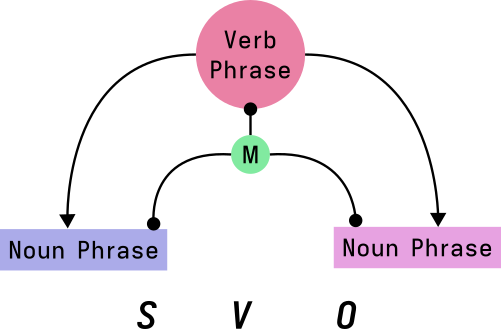
\includegraphics[width=\textwidth]{graphics/typical-sentence-structure.png}
    \caption{Typical sentence structure}
\end{figure}

modifiers that sentences as a whole are called sentence modifiers. sentence level modifiers usually appear at the beginning of a 
sentence and are separated by a comma.

\begin{enumerate}
    \item \emph{Understandably}, Sam decided not to come.
    \item \emph{On Thursday night}, Raymond bereated Madeline.
    \item \emph{Motivated by fear}, the squirrel scampered.
    \item \emph{Please}, wear you masks.
    \item \emph{Astoundingly}, the ice cream brought about world peace.
    \item \emph{Under duress}, we confessed to dismantling the planes.
    \item \emph{Responding to the news}, the detective threw a fit.
    \item \emph{When I was a child}, my father gave me licorice.
\end{enumerate}

sentence number 3 is an example of multi-word modifier. sentence number 6 is an example of sentence modifier that is prepositional
phrase. sentence number 7 is an example of sentence modifier that is participal phrase. the place of modifiers matters a lot.

\begin{itemize}
    \item \emph{Really}, the old touscan shrieked loudly at the miserable goose.
    \item The \emph{really} old touscan shrieked loudly at the miserable goose.
    \item The old touscan \emph{really} shrieked loudly at the miserable goose.
    \item The old touscan shrieked \emph{really} loudly at the miserable goose.
    \item The old touscan shrieked loudly at the \emph{really} miserable goose.
\end{itemize}

sentence can be made out of single verbs \emph{Stop!}, single independent clause that contains noun phrase and verbe phrase 
\emph{Each of the students leaving the classroom are pathetic loosert indefinately.} or from subordinated and independent clauses
\emph{After I told him to cut it out, Schmitt began to make more scene.}. Subordinating clauses begin with words known as 
subordinatiing conjunctions. \emph{After}, \emph{Because}, \emph{Although}, \emph{Despite} are example of subordinating conjunctions.

\{After the miserable party ended\}, [Georgio boldly declared that he was the  checkers champion], [but Lydia,
        incensed by the presumption, rejected his claim and proposed a board game coup\footnote{
            \emph{rejected his claim and proposed a board game} is a single verbal phrase with two objects attached.}]
\{because she saw her opportunity to prevail\footnote{subordinated clauses can come after the independent clause}\}. in the 
above complex sentence, subordinated clauses are in \{\} and independent clauses are in [].


\begin{figure}[hbt!]
    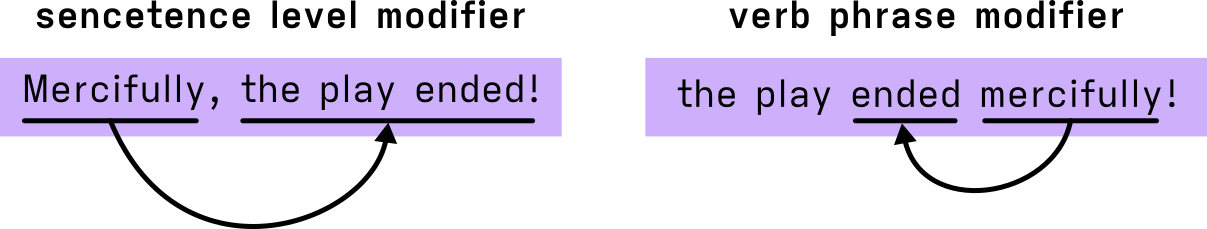
\includegraphics[width=\textwidth]{graphics/sentence-modifier.png}
    \caption{Sentence level and verb phrase modifiers}
\end{figure}

\begin{flushleft}
    Comma usage recorded thus far:
    \begin{enumerate}
        \item After sentence level modifiers.
        \item After subordinated clauses.
        \item Between independent clauses conjugated with one of FANBOYS.
    \end{enumerate}
\end{flushleft}

there is no agreed upon idea of what a paragraph should contain. paragraph is what start on indented line and ends a line white space.
aggregation of words into whitespace separeted bunches makes paragraphs a contained unit of language.
readers expect some from of structure from each of our paragraphs. \emph{Focus} is the most expected from the paragraphs we write.
each paragraph should talk about one idea only. \emph{Topic sentences} at the start of a paragraph orient our readers on what is to 
follow in the paragraph so they know what expect and can follow easily. we can think of topic sentences as labels for a paragraph.
human have a small working memory. make paragraph shorters and concise. a good \emph{flows}. By flow, we mean sentences in the paragraph
chain together to create effortless reading experience.


\section*{Deutsch}
\subsection*{Phonology}
Phonolgy is grammar of the sounds of a language, but phonetics is the study of human produced sound for its own sake.

the text bellow contains the translation of Rammsteins hit ich will.

\textsf{
    \begin{poem}
        ich will \\
        ich will \\
        ich will \\
        ich will \\
        ich will \\
        ich will \\
        ich will \\*
    \end{poem}
}
\emph{ich} is the first singular personal pronoun in the nominative case. the nominative case marks the subject of a verb.
the ohter cases of the first person singular personal noun are \emph{mich}, \emph{meiner}, \emph{mir} for accusative, genitive, and dative
cases repectively. \emph{will} is the singular first person present conjugation of \emph{wollen}. \emph{ich will} translated to english
means \emph{i want}.

\begin{table}
    \begin{center}
        \textsf{
            \begin{tabular}{l l r}
                \toprule
                Infinitive                     &     & \emph{wollen} \\
                \midrule
                \multirow{7}{*}{Present tense} & ich & will          \\
                                               & du  & willst        \\
                                               & es  & will          \\
                                               & wir & wollen        \\
                                               & ihr & wollt         \\
                                               & Sie & wollen        \\
                                               & sie & wollen        \\
                \midrule
                \multirow{7}{*}{Past tense}    & ich & wollte        \\
                                               & du  & wolltest      \\
                                               & es  & wollte        \\
                                               & wir & wollten       \\
                                               & ihr & wolltet       \\
                                               & Sie & wollten       \\
                                               & sie & wollten       \\
                \midrule
                \multirow{1}{*}{Participle}    &     & gewollt       \\
                \bottomrule
            \end{tabular}}
        \caption{\emph{wollen} conjugations.}
    \end{center}
\end{table}


\textsf{
    \centering
    \begin{poem}
        Ich will dass ihr mir vertraut \\
        (Ich will) Ich will dass ihr mir glaubt \\
        (Ich will) Ich will eure Blicke spüren \\
        (Ich will) jeden Herzschlag kontrollieren \\
        (Ich will) eure Stimmen hören \\
        (Ich will) Ich will die Ruhe stören \\
        (Ich will) Ich will dass ihr mich gut seht \\
        (Ich will) Ich will dass ihr mich versteht \\*
    \end{poem}
}

\emph{dass} is a subordinating clause introducer similar to english's \emph{that}. \emph{eure} is the genitive of the second person 
plural \emph{ihr} (you (all)). \emph{jeden}\footnote{except that jeden (rather than jedes) is usual in the genitive
    singular masculine and neuter if the following noun has the ending -(e)s, e.g.
    \emph{am Ende jed \textbf{en}} (less frequent: \emph{jed \textbf{es}}) \emph{Abschnitts.}} is a determiner that corresponds to
english \emph{each}, \emph{every}. \emph{kontrollieren}

\begin{table}
    \centering
    \textsf{\begin{tabular}{l l l r}
            \toprule
                       & Masculine      & Feminine & Neuter \\
            \midrule
            Nominative & jeder          & jede     & jedes  \\
            Accusative & \textbf{jeden} & jede     & jedes  \\
            Genitive   & \emph{jedes}   & jeder    & jedes  \\
            Dative     & jedem          & jeder    & jedem  \\
            \bottomrule
        \end{tabular}}
    \caption{Declension of \emph{jeder}}
\end{table}

\textsf{
    \centering
    \begin{poem}
        I want that you (all) trust me \\
        (Ich will) I want that you (all) believe me \\
        (Ich will) I want your glancing look. \\
        (Ich will) Each heartbeat controlling. \\*
    \end{poem}
}

\begin{figure}
    \centering
    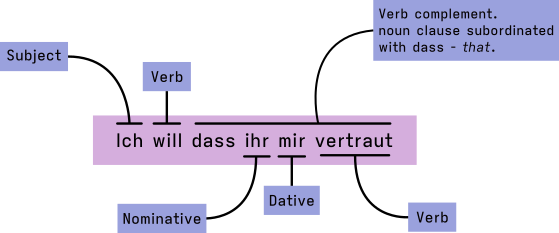
\includegraphics[width=\textwidth]{graphics/grammar-syntax.png}
    \caption{Verb structure for the first verse}
\end{figure}

\begin{figure}[hbt]
    \begin{center}
        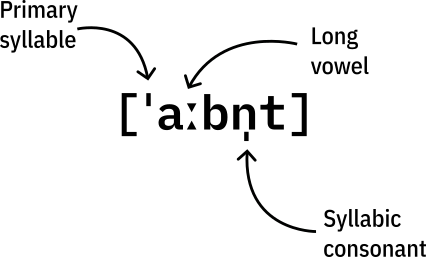
\includegraphics[width=0.5\textwidth]{graphics/ipa.png}
        \caption{IPA symbols.}
    \end{center}
\end{figure}

\subsection*{Grammar}
All german nouns are ``gendered''. the genders are: neutral, male and female. but the actual gender of the noun has
nothing to do with its gender especially for inanimate objects. german nouns are to be memorized with the 
article reflecting the gender. These are \emph{der}-nouns (masculine), \emph{die}-nouns (feminine) and \emph{das}-nouns 
(neuter). Examples: \emph{das Cafe}, \emph{der Flughafen}, \emph{der Banhof}, \emph{das Restaurant}, \emph{das Hotel},
\emph{die Botschaft}, \emph{die Bank}, \emph{die Zigarren}, \emph{der Wein}, \emph{das Bier}, \emph{der Kaffe},
\emph{der Tee}, \emph{die Milch}, \emph{das Wasser}, \ldots It makes no sense for wine to a masculine gender.

\subsubsection*{Personal pronouns}

\begin{table}[hbt!]
    \centering
    \textsf{\begin{tabular}{ l l l r }
            \toprule
            Nominative & Accusative & Genitive & Dative \\
            \midrule
            ich        & mich       & meiner   & mir    \\
            du         & dich       & deiner   & dir    \\
            er         & ihn        & seiner   & ihm    \\
            sie        & sie        & ihrer    & ihr    \\
            es         & es         & seiner   & ihm    \\
            wir        & uns        & unser    & uns    \\
            ihr        & euch       & euer     & euch   \\
            Sie        & Sie        & Ihrer    & Ihnen  \\
            sie        & sie        & ihrer    & ihenen \\
            \bottomrule
        \end{tabular}}
    \caption{Personal pronouns in Deutsch.}
\end{table}


Unlike Enlgish verbs which are only conjugated for number, and tense, German verb conjugation depends on number, gender, 
person, mood, and tense. German verbs can be regular or irregular in their conjugation. Finite verbs must agree with
the subject, unlike non-finite verbs.

The ``principal parts'' of a verb are:
\begin{enumerate}
    \item Infinitive form.
    \item Past tense form.
    \item Past participle form.
\end{enumerate}

Based on conjugation I need to worry about:

\begin{enumerate}
    \item Weak verbs.
    \item Strong verbs.
    \item Irregular verbs.
          \begin{enumerate}
              \item Irregular weak verbs.
              \item Irregular strong verbs.
              \item The modal auxiliary verbs and \emph{wissen}.
              \item The verbs \emph{haben}, \emph{sein}, and \emph{werden}.
          \end{enumerate}
\end{enumerate}

\begin{figure}
    \centering
    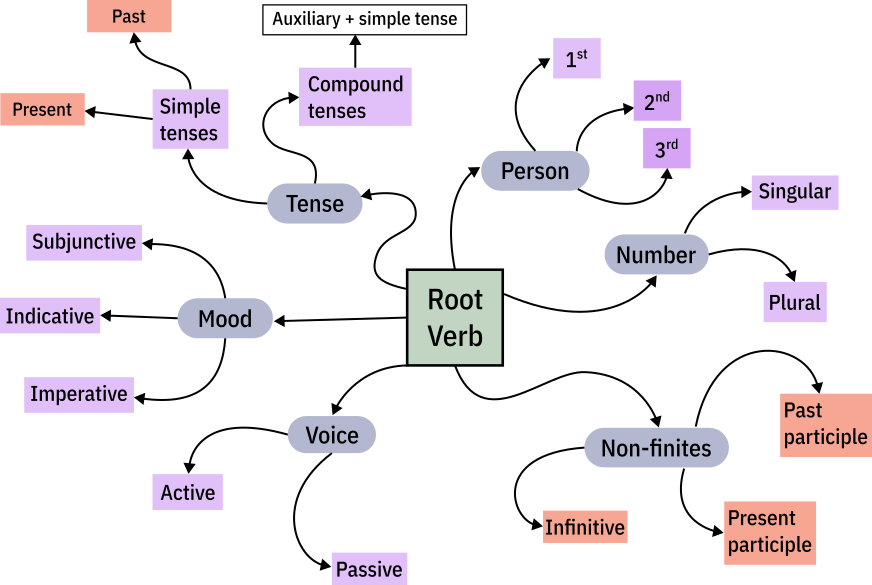
\includegraphics[width=0.85\textwidth]{graphics/german-verb-conjugation.png}
    \caption{German verb conjugations}
\end{figure}

\section*{Java notes}

\subsection*{Type theory interlude}

\subsubsection*{Subtyping}

In programming language theory a \emph{subtype} referes to a a type that is related to another type, also called the 
\emph{supertype}, by some notion of \emph{substiutability}, meaning that program elements typically functions (or subroutine)
written to operate on the supertype can also operate on the subtype. If \(S\) is the subtype of \(T\), the subtyping relation
is often written as \(S <: T\), to mean that any term of type \(S\) can safely be used in places that expect type \(T\) to be
present. For example in Java, every type except for primitive types is the subtype of \lstinline{Object} class. Or stated
mathematically:
\[
E <: O  
\]
Where E is every other class and O is the \lstinline{Object} class. 

\subsubsection*{Covariance, contravariance, and invariance}
\emph{Variance} refers to how the subtyping of more complex types is related to subtyping between the component types.
Complex types include: generics, functions, and collections types like arrays, maps, and linked lists. For example, 
should \lstinline{List<Cat>} be the subtype of \lstinline{List<Animal>} give that type \lstinline{Cat} is the subtype of type \lstinline{Animal}? Does
\[L[C] <: L[A]\] hold given that \[C <: A\] for a given programming language like Java? Since Java supports generics, which
allow the programmer to extend the type system with new type constructors (parametric polymorphism), which raises the question
should \lstinline{ArrayList<File>} be the subtype of \lstinline{ArrayList<Object>} (\emph{covariant})? Java uses 
\emph{use-site}  annotation to describe the varaince of the generic type constructors. \emph{declaration-site} annotation is
used by C\#, Kotlin, and Scala. 

Within a type systm of a programming language, a type rule or a type constructor is:

\begin{itemize}
    \item \emph{covariant} if it preserves the ordering of types (\(\leq\)), which orders types from more specific to more
          generic: If \(C <: A\), then \(I[C] <: I[A]\).
    \item \emph{contravariant} if it reverses this ordering if \(C <: A\), then \(I[A] <: I[C]\).
    \item \emph{bivariant} if both of this apply. (i.e., if \(C <: B\), them \(I[C] \equiv I[A]\)).
    \item \emph{variant} if covariant, contravariant, or bivariant.
    \item \emph{invariant} or \emph{nonvariant} if not variant.
\end{itemize}

\subsection*{Package management}
Classes live inside packages. a package declared using \lstinline{package ...;} classes living in the same 
package can see each other. package \emph{classpath} and directory structure of the source must match each other. 
always think of two contexts the classpath context and source context. why should java source directory tree and
package name classpath match? answer here. relationship with maven group id and artifact ids?

\subsection*{The language}

Non wildcard (\lstinline{G<?>}) parameterized types are invariant in Java, i.e, there is no subtyping relationship between
\lstinline{List<Cat>} and \lstinline{List<Animal>}. \footnote{more on this.}

Java does not suffer from template bloat like C++ does. Why? That is because C++ creates a new type for every template 
instantiation. For example:

\lstset{style=custom-cpp}
\begin{lstlisting}
    template <typename T>
    void print(T arg) {
        // ... implementation
    }

    print<int>(30);
    print<const char*>("Hello");
\end{lstlisting}

Essentially generates two copies of the function print with the type paramenters resolved: \lstinline{printInt} and
\lstinline{printConstPtrToChar} which generates bloat during compilation. Java unlike C++ generates just one type for each
generic type with the generic type thrown away, which call \emph{type erasure}.

\lstset{style=custom-java}
\begin{lstlisting}
    public <T> void print(T arg) {
        // ... implementation
    }
\end{lstlisting}

\begin{flushleft}
    becomes just one function with type parameters replaced with \lstinline{Object} type.    
\end{flushleft}

\begin{lstlisting}
    public void print(Object arg) {
        // ...implementation
    }
\end{lstlisting}

\subsection*{Dependency injection}

Dependency injection is a design pattern applied to classes with members so that the member are initialized outside the class
itself. For example, the following code:

\lstinputlisting[style=custom-java]{code/code-without-di.java.src}

\lstinline{RealBillingService} class depends on two internally constructed objects inside the \lstinline{chargeOrder}
function. If we wanted to test \lstinline{chargeOrder}, we will have to charge from a real Paypal account which is
impractical. To solve this we could use:

\begin{itemize}
    \item Using a Factory class but we would have to reset this global factory after each test.
    \item Passing every dependency to constructor manually. using method we can remove \lstinline{setUp} and \lstinline{tearDown}
          methods from our test code. further more expose the dependency in the api signature.
    \item Using a dependency injection framework.
\end{itemize}

Java is getting better and better with each release. Keep the the features listed below in mind when working with a new
java project.
\begin{itemize}
    \item better \lstinline{switch} blocks.
    \item a smarter \lstinline{instanceof} operator.
    \item Records with autogenerated getters, setters, and to string.
    \item Text blocks.
    \item sealed classes.
\end{itemize}

\subsection*{Java security primitives}
Java uses serveral classes and interfaces from core java packages to thrid party libraries to help with the control of \emph{access to information}.
\emph{Principal} interface represents an abstract notion of a principal, which can be used to represent any entity, 
such as an individual, a corporation or a login id. Essentially, anything with a name (that name could be a user id from user database) 
is principal. 
A \emph{Credential} is a piece of document that details the qualification, competence, or authority issued to an individual by a third party
with a relevan defacto authority assumed competence to do so. Examples of credentials include academic degrees, passwords,
security clearance, badges, passwords, user names, keys, and certifications. \emph{Subject} \lstinline{class} represents 
a \emph{grouping} of related information for a single entity, such as a person. Such information includes subjects indentities
as well as security related attributes (passwords, cryptographic keys, for example.) Subjects may potentially have multiple
indentities. Each identity is represented as a \lstinline{Principal} within the \lstinline{Subject}. For example a \lstinline{Subject},
that happens to be a person, Alice, might have two principals: on which binds ``Alice Bar'', the name of her driver license,
to the \lstinline{Subject}, and another which binds ``999-99-999'', the number of her student identification card, to the 
\lstinline{Subject}. Both \lstinline{Principal}s refer to the same \lstinline{Subject} even though each has different name. 


\lstset{style=custom-java}
\begin{lstlisting}
    package java.security;

    public interface Principal {
        // ...
        String getName();
        boolean implies(Subject subject);
        // ...

    }
\end{lstlisting}

\subsection*{Important Java foundations}
The Eclipse foundation and Apache foundation contribute a great deal to the advancement of the Java ecosystem.
Besides that Red Hat and Oracle are commercial companies engaged in the development and support of Java Platform.

\subsection*{Jakarta EE}
Jakarata EE also previously known as Java Enterprise Edition is a set of \emph{Specifications} that extend Java SE
with specifications for enterprise features such as distributed computing and web services. Jakarata EE defined by 
its specification, and its specification defines APIs and their interaction. Jakarta EE was maintained by Oracle
corporation who later transffered its development to Eclipse foundation was renamed from Java EE to Jakarta EE because
Oracle owns the trademark for \emph{Java}. 

\subsection*{OSGi}

OSGi specification describes a modular system and service platform for Java that implements a complete and 
dynamic component model, something that does not exist in standalone Java/VM platforms. In enterprise settings typical 
Java application is not packaged as jar and launched from its main function using the system installed java executable,
rather than that the enterprise system provides a java platform that \emph{always} runs in which application bundles are
loaded and unloaded with out restarting the application server. OSGi architecture has the following components:

\begin{enumerate}
    \item \emph{Bundles} are normal JAR components with extra manifest headers.
    \item \emph{Services} layer connects bundles in a dynamic way by offering a publish-find-bind model for POJIs and POJOs.
    \item \emph{Service registry} the application programming interface for management services.
    \item \emph{Life-cycle} the application programming interface for lifecycle management (insatll, start, stop, update, uninstall)
          for bundles.
    \item \emph{Modules} layer defines encapsulation and declaration of dependencies (how bundles can import and export code).
    \item \emph{Security} layer that handles the security aspects by limiting bundle functionality to pre-defined capabilities.
\end{enumerate}

\emph{Apache Felix} is implementation of the OSGi specification.

\begin{figure}[hbt]
    \begin{center}
        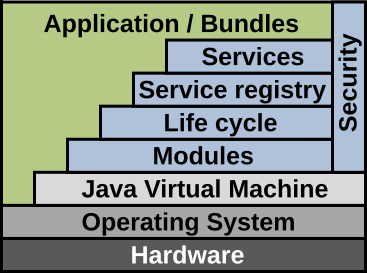
\includegraphics[width=0.5\textwidth]{graphics/osgi-architecture.png}
        \caption{OSGi architecture.}
    \end{center}
\end{figure}

\subsection*{Glassfish}


\subsection*{JAX-RS}
Jakarta RESTful Web Services also called \emph{JAX-RS} is a set of interfaces and annotations included in Java EE platform 
that help in writing REST applications. Since JAX-RS is just a collection of interfaces and annotations it just defines an API. 
RestEasy from Red Hat, Jersey from Eclipse foundation and Apache CXF are the libraries implementing the API.

\emph{Root resource classes} are POJOs that are annotated with \lstinline{@Path} have atleast one method annoted with
\lstinline{@Path} or a resource method designator annotation such as \lstinline{@GET}, \lstinline{@POST}, \lstinline{@PUT},
or \lstinline{@DELETE}. Resource method are methods of resource class that are annotated with resource method designator.

Java world is full of specifications and implementations (some of which are reference). Language features such as interfaces, 
annotations and abstract base classes aid writing specifications in java code.

%% a section that describes the working of traccar server.
\subsection*{The server}

Traccar server is a 3 layer monolithic application where each layer handles a specific functionality\footnote{
    If this is the topic sentence, then the rest of the paragraph should be about some sort of layering.
}. The top layer in the application receives incoming request from mobile and application clients as well as both http and websocket
connection. The middle layer of the application processes these requests and performs business logic before the third layer
persists or reads objects to a database. 

The top layer of Traccar is composed of a set of servlets. One of the servlets handles incoming REST API (Application Programming 
Interface) calls from mobile and web clients. The other servlets handle websocket communication with tracking devices and serving
media files for web clients. Since almost all of our modification is related to business logic and authorization related stuff,
we will focus on the REST API servlet.

The REST API servlet implements the Jakarta RESTful Web Services (JAX-RS) specification. JAX-RS specification provides its 
users with annotations to decorate their classes. Traccar server uses Eclipse Jersey as the implentation library of JAX-RS. REST API 
resources are bound to handler classes with annotations. Each handler class is annotated with REST API resource \emph{path}. Annotated 
functions in the resource class handle specific HTTP methods. This layer of the application is commonly called the controller. Jersey 
takes FasterXML's Jackson JSON serialization/deserializtion library in its filter chain to convert incoming JSON payloads to the 
application objects. 


Before each request is received by the resource handler classes, it passes through a class that implents JAX-RS' 
\lstinline{ContainerRequestFilter} interface. This interface contains the \lstinline{filter} function. 
The \lstinline{filter} function allows us to perform custom logic on all requests before they are matched with and dispatched to our 
resource handler classes. Our implementation of the interface checks if each request contains a JSON Web Token 
(JWT) payload in the \lstinline{Authorization} header, and If the header is present it tries to decode it and retrieve a valid Firebase
user using Firebase Admin library functions.

Another function of our class implementing \lstinline{ContainerRequestFilter} is to inject objects that are usefull for processing
incoming requests. It injects a \lstinline{SecurityContext} object for use by our resource handler classes. The injected object 
contains authentication information necessary for the logic inside our resource handlers. One such information is the user's unique 
identifier ID decoded from the JWT payload.

\lstinline{Storage}  class is also injected into the resource handlers. \lstinline{Storage} interfaces with the underlying database 
to write and read application objects in memory. Connection to the underlying database is managed by HikariCP connection pool 
management library. We manage our connections with HikariCP because we want to be resource efficient. We become resource efficient by not 
recreating database connection for every request but by storing and reusing connections from older completed requests. By doing 
connection pooling, we reduce object creation/destruction overhead. 

Traccar server uses Liquibase database migration tool to automatially initialize tables on startup. Liquibase reads table creation 
data from \emph{schema} files written in XML. Each schema file is written in the from of \emph{changesets}. changesets help us in 
the process of restoration of older database state. Traccar server uses a custom Object Relational Mapping (ORM) system. 
Each Traccar model class we want to persist is annotated with \lstinline{@StorageName}. \lstinline{@StorageName} helps the ORM to 
generate column names and table names using Java's support for runtime reflection. By using annotations and reflection, we can load 
database table rows to application memory objects of a classes that are annotated with \lstinline{@StorageName} or insert objects that 
are annotated with \lstinline{@StorageName("table_name")} to database rows. Each of the API handlers use instance of  
\lstinline{Storage} class to read and write persistance data. 

\emph{Data managers} sit between \lstinline{Storage} class and our resource handlers to facilitate the 
implementation of a more complex logic. This more complex logic is usually a code that shares functoinaliy with the websocket code. 


Objects in Traccar server are linked with each other post creation. Special tables in the database store this linkage information. 
\lstinline{Permission} model class helps when linking objects together.\footnote{how?}. \lstinline{PermissionService} class is also injected 
for use by resource handler classes. \lstinline{PermisssionService} class handles various authorization related functionalities. 
Authorization related function include: check if user is admin, check if users can access reports, check if a give user can edit or 
update database objects, check if a given user owns certain model classes, etc\ldots


\begin{sidewaysfigure}[hbt!]
    \centering
    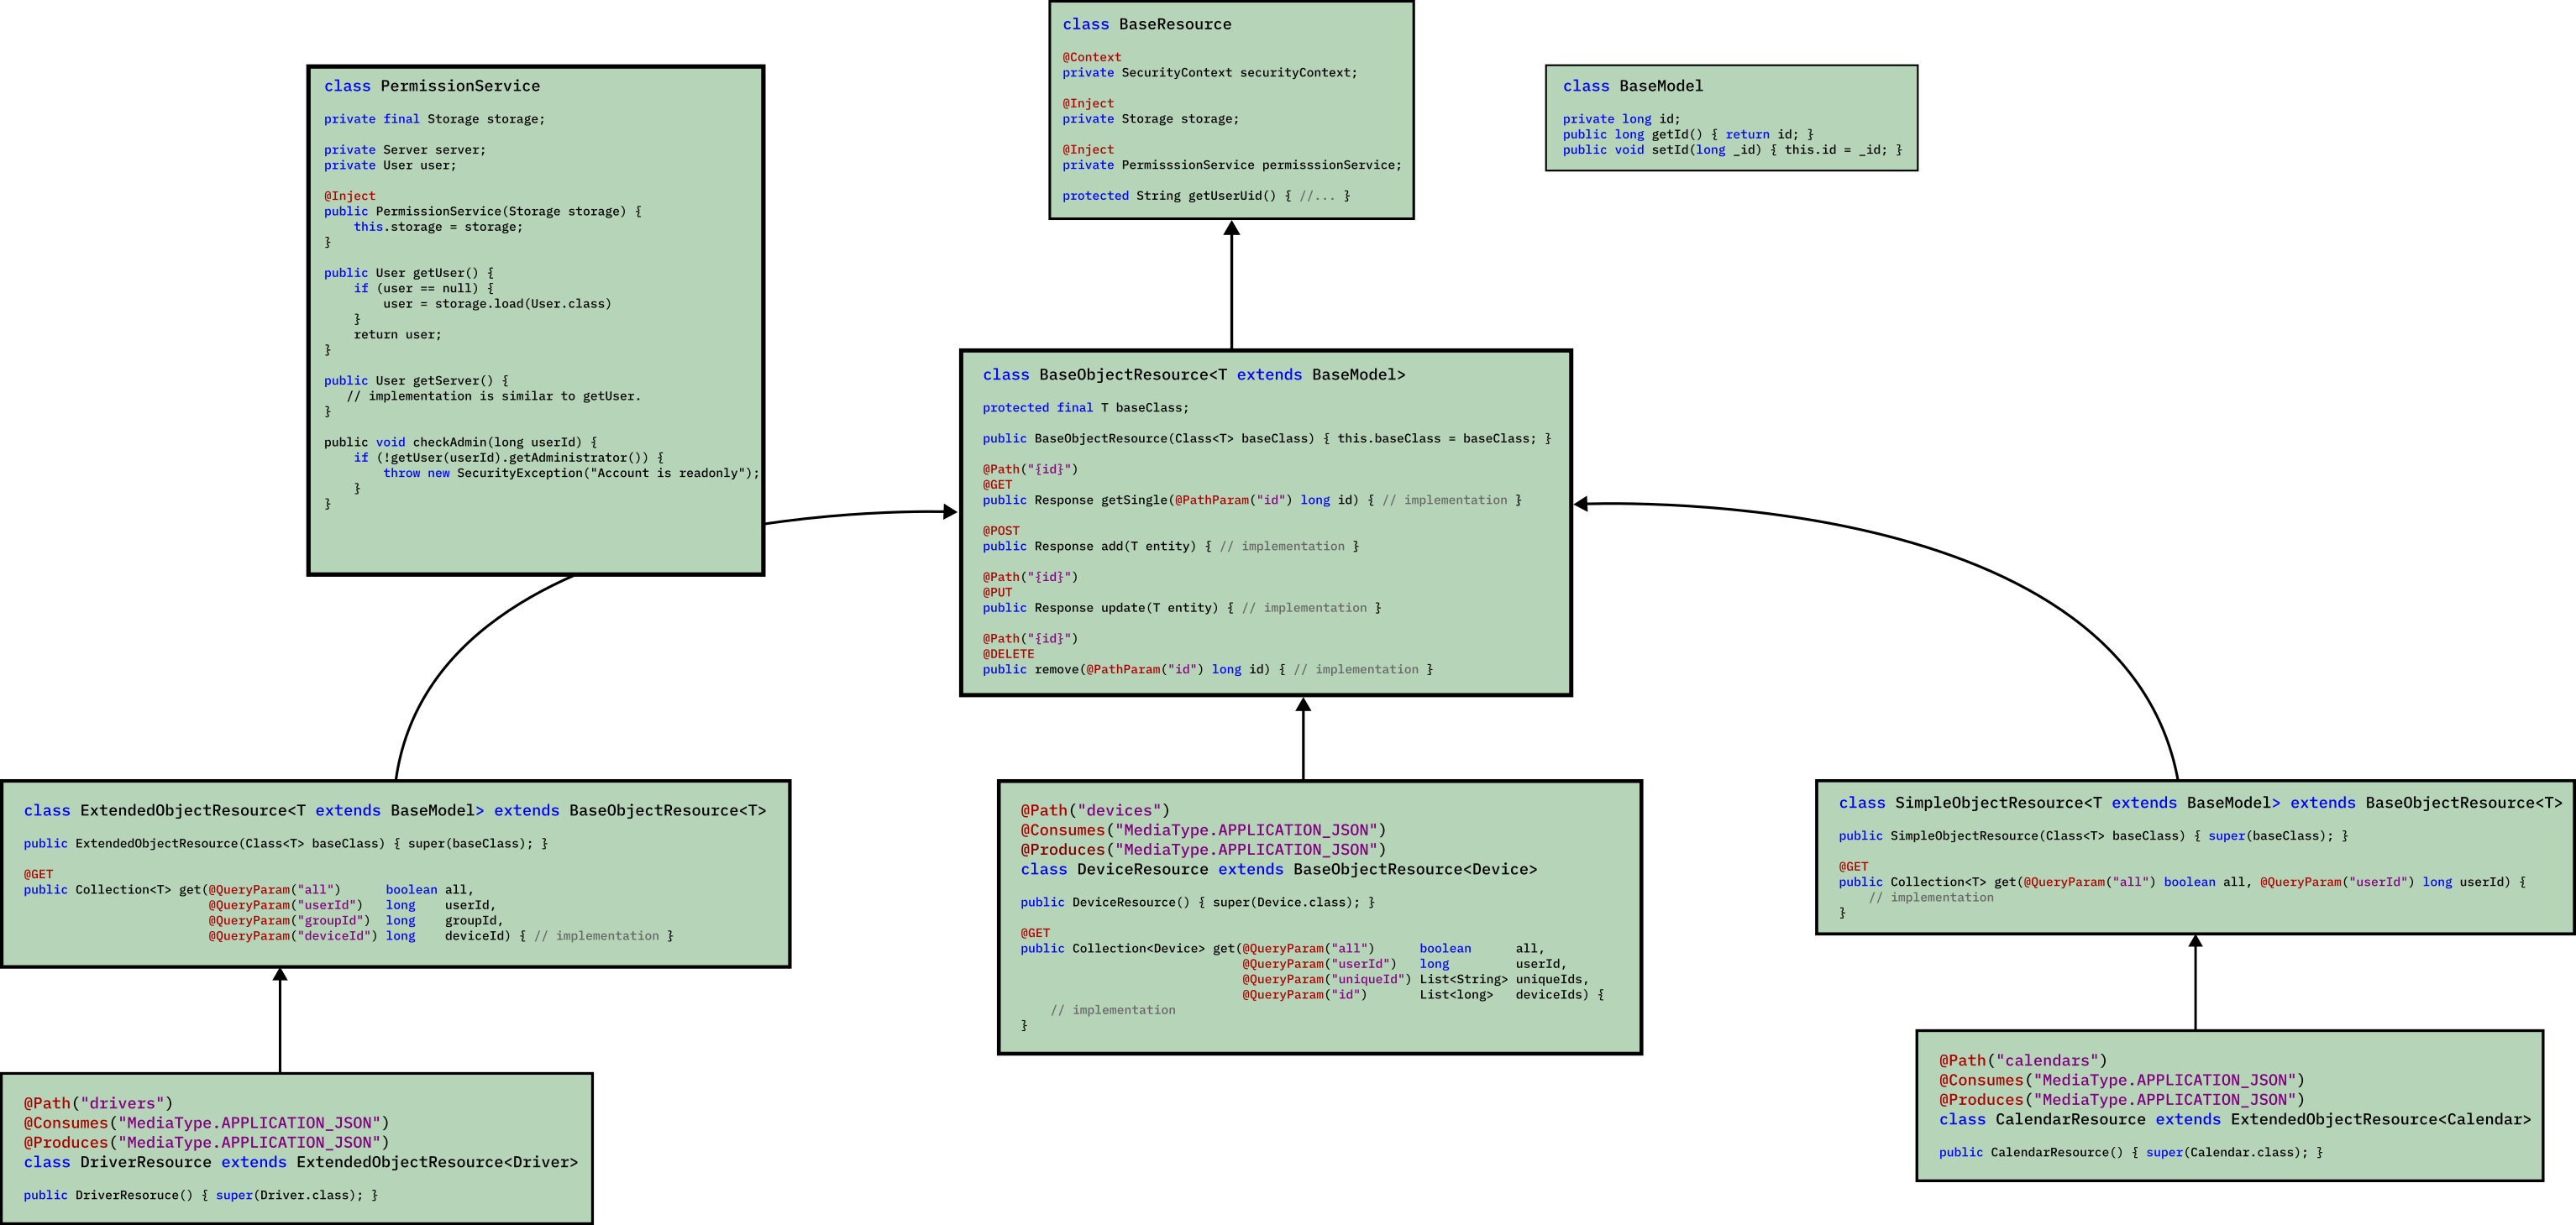
\includegraphics[width=\textheight]{graphics/uml-chart.png}
    \caption{Traccar UML chart}
\end{sidewaysfigure}

\section*{SQL notes}

\lstset{style=custom-sql}

Why did relational databases win out? Database is a \emph{set} of related information\footnote{Learning SQL}. Databases can
be indexed with some \emph{key}. A phonebook has letters on its margins. We can use the letters on the margins to find
phonenumbers quicker. We call this process \emph{indexing}. relational mode of data storage is the most commonly used.
heirarchial mode of data storage was more popular in the past. in heirarchial data storage scheme data is stored in a tree 
fasion. as an example of heirarchial data storage we can consider the case of bank account storage.

\begin{figure}[hbt!]
    \centering
    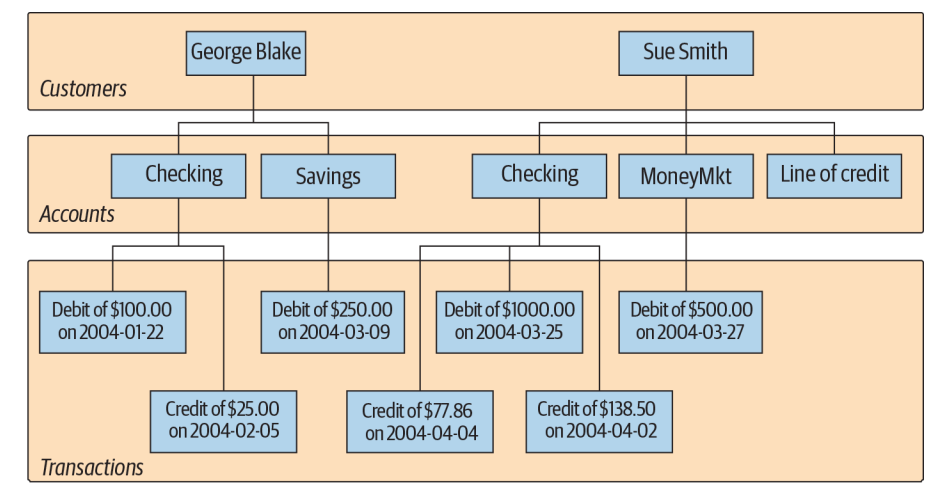
\includegraphics[width=0.5\textwidth]{graphics/heirarchial-database.png}
    \caption{Heirarchial mode of data storage.}
\end{figure}

network based database store records with pointers to other records. user can extract data by traversing the linking pointers.
relational database is the most common now. primary keys uniquely identify a row in relational table. primary keys need not be
generated by the database management software. several columns can generate a unique key for each row. \lstinline{fname} and
\lstinline{lname} in the database attached can be used as a primary key. primary keys made out of multiple columns are called
\emph{compound key}. \emph{natural keys} are keys generated from the data itself. \emph{surrogate keys} are keys appended 
by the database designer. database designers generate surrogate primary keys because no natural key can be used to identify
a row. primary keys should never change once they are assigned. relational database tables include column whose value point
to entries in other tables. column value that point to another table are called foreign keys. foreign keys perform the same
function as pointers in network based database systems.the process of ``lensing'' into foreign key of table is called a
\emph{join operation}. storing redundant is not considered a problem in relational database system. we must be sure that 
redundant data stored has a reason to be redundant. cannonical data should be stored in one table. foreign keys (pointers)
can be redundant. duplication of cannonical data causes for unreliable data. a single column should just include one data.
this process of making cannonical data non redundant, storing single values in each column is called \emph{normalization}.
sql is a computer language that was specifically designed to manipulate relational databases. Edgar F. Todd described relational
database systems. he proposed a language called DSL/Alpha for relational database systems. IBM created a language called 
SQUARE by refining edgar f. codds language. SQUARE was refined to SEQUEL. SEQUEL was shorted to SQL. The result of sql query 
is a table. a new table can be created in sql by simple storing the result set of an sql query. a query can use both permanent
tables and result set of another query. sql is not an acronym for anything. sql is short for sequel. sql is a non procedural
computer language. we do not tell the sql engine how to retreive our data. we describe the data we want to the sql engine and
the sql engine retreives the data the most efficient way possible. sql statement types can be divided into three types. 
\emph{schema statements} are used to define data structures stored in the database. \emph{data statements} are used to manipulate 
data structures created by schema statements. transaction statements are used to begin, end, and rollback transactions. 
an example of a the schema statement \lstinline{create table}:

- temporal data types.
- constraints, especially foreign ones.
- table joins.

\begin{figure}[hbt!]
    \centering
    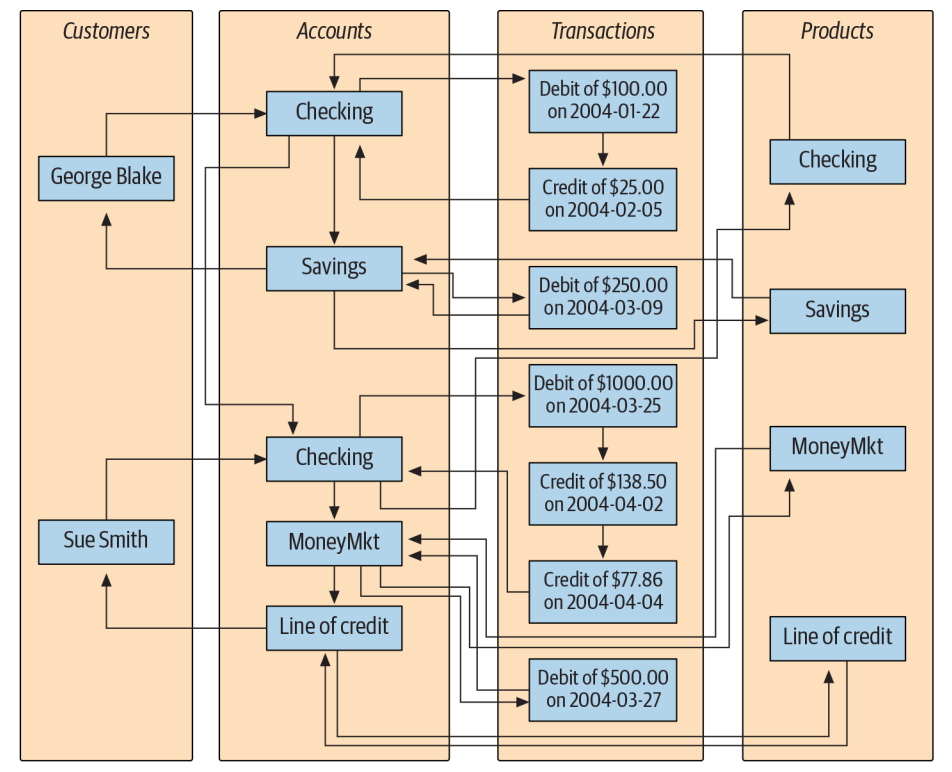
\includegraphics[width=0.5\textwidth]{graphics/network-database.png}
    \caption{Heirarchial mode of data storage.}
\end{figure}

\begin{lstlisting}
create table corporation (corpid smallint, name varchar(30), constraint pk_corporation primary key (corp_id));
\end{lstlisting}

the above statement creates a table with two columns. the tables names is corporation. \lstinline{corp_id} is identified as the 
primary key. primary keys are a type of constraint. \lstinline{insert} is a data statement that is used to insert a row of data into
a table. notice the single quote in insert.

\begin{lstlisting}
insert into corporation (corpid, name) values (30, 'SpaceX');
\end{lstlisting}

another data statement is \lstinline{select} statement. \lstinline{select} statement is used to extract data from the database.

\begin{lstlisting}
select (name, corpid) from corporation where corpid=30;
\end{lstlisting}

all database elements created with sql schema statements are stored in a set of special tables called \emph{the data dictionary}.
this set of metadata tables can be queried just like other sql tables.

several \emph{clauses} make up a query statement. only \lstinline{select} is mandatory for a query statement. \lstinline{select}
clause runs last after filtering, grouping and ordering operations. instead of just \emph{selecting} rows from operation of other
claues, for example \lstinline{from} clause's, \lstinline{select} clause can add synthetic rows to the result set. we can think of
like the other clauses providing \lstinline{select} for columns to select from. \lstinline{as} introduces a column alias.
\lstinline{from} clause defines the tables used by a query, along with the means of linking tables together. \lstinline{from} clauses 
are very important for table join operations.

\begin{lstlisting}
-- select every column from language table for the result set.
select * from language;

-- select just language_id and name from language table for the result set.
select language_id, name from language;

-- select for 'synthetic' rows.
select 
    language_id as id, -- id is a column alias for language_id
    'COMMON' as language_usage, -- 'synthetic' row
    language_id * 3.1415927 as lang_pi_value, -- 'synthetic' row
    upper(name) as language_name, -- 'synthetic' row
    version() as version -- or even this!
from 
    language;
\end{lstlisting}

\flushleft\lstinline{from} clause can take various forms of tables:

\begin{enumerate}
    \item \emph{Permanent tables} created with \lstinline{create table}.
    \item \emph{Derived tables} retured from a subquery and held in memory.
    \item \emph{Temporary tables} that are volatile tables held in memory.
    \item \emph{Virtual tables} created with \lstinline{create view} statement.
\end{enumerate}

\begin{lstlisting}
select
    concat(cust.last_name, ', ', cust.first_name) as full_name
from -- from clause taking in a drived table.
    (select
        first_name,
        last_name,
        email
    from
        customer as c
    where
        c.first_name = 'JESSIE') as cust;
\end{lstlisting}

\begin{table}[hbt!]\sffamily
    \begin{center}
        \begin{tabularx}{0.75\textwidth}{l X}
            \toprule
            Clause name          & Purpose                                                                               \\
            \midrule
            \lstinline{select}   & Determines which query to include in the query's result set                           \\
            \lstinline{from}     & Identifies the tables from which to retrieve data and how the tables should be joined \\
            \lstinline{where}    & Filters out unwanted data                                                             \\
            \lstinline{group by} & User to group rows together by common column values                                   \\
            \lstinline{having}   & Filters out unwanted groups                                                           \\
            \lstinline{order by} & Sorts the rows of the final result set by one or more columns                         \\
            
            \bottomrule
        \end{tabularx}
        
        \caption{Query clauses}
    \end{center}
\end{table}

\lstinline{from} clauses can also choose from 2 or more tables. by default from statement with out a join type will perfrom cross 
product for each row of all the columns of table A with all columns of table B. table joins can be chained together for more than
two tables.

\begin{lstlisting}
select
    concat(cu.first_name, ' ', cu.last_name) as name, ct.city
from
    customer as cu 
    inner join address as ad 
        on cu.address_id = ad.address_id 
    inner join city as ct 
        on ad.city_id = ct.city_id;
\end{lstlisting}

one unique cutomer (by definition) can have multiple rental records. this, we call one-to-many relationship.

\begin{figure}
    \centering
    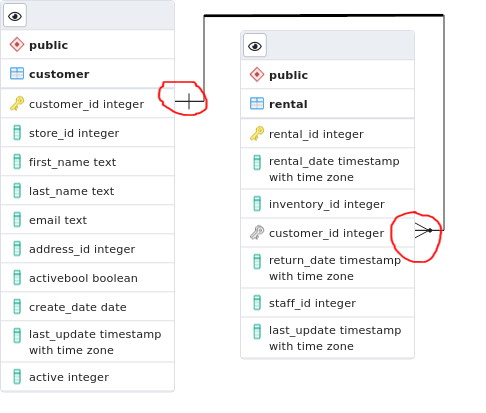
\includegraphics[width=0.6\textwidth]{graphics/one-to-many-relationship.jpg}
    \caption{One to many relationship in tables}
\end{figure}

\lstinline{group by} collects collects rows by equality of rows we provide. \lstinline{count(column)} stores how many there are in a 
group.

\begin{lstlisting}
select
    f.film_id, f.title, count(*) num_copies
from
    film as f 
        inner join inventory as i 
        on f.film_id = i.film_id
group by
    f.film_id, f.title;
\end{lstlisting}

\lstinline{inner join} truncates rows that are not in both tables based on the condition we provided. to include rows of one table
no matter what, we employ \lstinline{outer join}.

\begin{lstlisting}
select
    -- note: count(i.inventory_id)
    f.film_id, f.title, count(i.inventory_id) num_copies
from
    film as f
    left outer join inventory as i 
    on f.film_id = i.film_id
group by f.film_id, f.title
order by f.film_id;
\end{lstlisting}

\subsection*{PostgreSQL}
\lstset{style=custom-bash}
PostgreSQL is one of the most popular sql based database management systems. PostgreSQL is fully opensource. PostgreSQL is developed 
by Berkley University. installing posgresql on  an Arch Linux machine creates a \lstinline{postgres} user. \lstinline{postgres} user 
is the only one allowed to interact with the database system. to change to user postgres use the following command. command work 
if \lstinline{sudo} is installed. postgresql follows the client server model. postgresql server manages the datastore. postgresql 
server receives sql commands from clients and executes it against the datastore. servers and clients need not be on the same host.
server client can communicate using TCP/IP.


\begin{lstlisting}
sudo -iu postgres
\end{lstlisting}


then while we are user \lstinline{postgres}, initialize the database cluster with locale and encoding we desire.

\begin{lstlisting}
# initializes a database cluster.
# run as `postgres` unix user.
initdb  --locale=en_US.utf8 --encoding=UTF8 \
        -D /var/lib/postgres/data --data-checksums
\end{lstlisting}

PostgreSQL installs the following programs on our system: \lstinline{psql} is a postgresql client that helps us interact 
with PostgreSQL from a terminal session. \lstinline{createuser} is used to create PostgreSQL roles. \lstinline{postgres} is
used to manage the server process. \lstinline{initdb} is used to initialize database clusters. \lstinline{createdb} to create new
database (not a cluster). \lstinline{dropdb} to remove a database. commands from postgresql package must be run from the 
\lstinline{postgres} unix user. postgresql has the concept of roles. roles in postgresql are a username password combo that is
used to connect with a specific database. unix users and postgresql roles are a completely different concepts. a database client
from a remote machine can use a database installed locally by providing the correct roles. management of the database server is 
perfromed by \emph{unix} user \lstinline{postgres}. postgresql comes with one default role \lstinline{postgres}. \lstinline{postgres}
role is a super user role. super user roles can read and write to every database. super user roles can create and drop roles.
linux user \lstinline{postgres} and postgresql superuser role having the same name make things a little confusing. postgresql roles can
be create from the terminal using \lstinline{createuser} or from the interactive sql shell psql using sql statement:

we can connect to to database using superuser role \lstinline{postgres} from anywhere!

\lstset{style=custom-sql}
\begin{lstlisting}
create role dbname;
\end{lstlisting}

postgresql db roles can be removed using:

\begin{lstlisting}
drop role dbname;
\end{lstlisting}

\lstset{style=custom-bash}

Create a database for role \lstinline{dbname}.

\begin{lstlisting}
# create database named db for role dbname
# remember unix user is postgres
createdb db -O dbname
\end{lstlisting}

Then connect to the database using \lstinline{psql}

\begin{lstlisting}
psql db -U dbname
\end{lstlisting}

we will be presented with the following prompt.

\begin{lstlisting}
psql (14.3)
Type "help" for help.

db=> 
\end{lstlisting}

arrow instead of hash in \lstinline{db=>} indicates we are a non superuser role. contrast this with prompt for superuser role
\lstinline{postgres}:

\begin{lstlisting}
psql (14.3)
Type "help" for help.

db=#
\end{lstlisting}

we can use \lstinline{psql} command \lstinline{\dt+} to list all available tables in a database.

\section*{Algorithms}

\subsection*{What are algorithms?}

An \emph{algorithm} is is any well defined computational procedure that takes some value, as \emph{input} and produces some value, 
or a set of values, as \emph{output} in finite amount of time. Essentially algorithms are a set of procedures that transform input to outputs.
\footnote{As defined in the Algorithms book.}

Alternatively an algorithm can be described as a tool for solving a well defined \emph{computational problems}. The statement of problem describes
the desired input/output mapping for problem instances. The algorithm describes computational procedures for achieving the desired input/output relationship
for all problem instances.

Example problem: sort a sequence of numbers in ascending order. Below is how we formally define \emph{the sorting problem}.

Input: A sequence of \(n\) numbers \(\langle a_1, a_2, \ldots, a_n\rangle\). 

Output: A permutation (reordering) \(\langle a'_1, a'_2, \ldots, a'_n\rangle\) of the input such that \(a'_1 \leq a'_2 \leq \ldots \leq a'_n\).

\begin{itemize}
    \item a correct alogrithm should produce the correct output for each input but also halt. (finite running time.)
          \begin{enumerate}
              \item Prove that the algorithm actually \emph{works}.
              \item Analyze the running cost of the algorithm especially interms of order of growth.
          \end{enumerate}
    \item The example of comparision between a slow implementation of merge sort with cost of \(c_1n\lg{n}\) and insertion sort with running cost of
          \(c_2n^2\) is illuminating.
\end{itemize}

\section*{C++ notes.}

\subsection*{Smart pointers.}

I should avoid using raw pointers whenever possible. Why?
\lstset{style=custom-cpp}

\begin{itemize}
    \item Declaration does not indicate whether they point to a single object or an array.
    \item Declaration does not tell us whether a pointer should destroy the object it is pointing at i.e. it is owning.
    \item There is almost no way to know whether to call \lstinline{delete} or \lstinline{delete []} from its declaration.
    \item Pass the pointer to a dedicated destroy function or just \lstinline{delete} it? Hard to know.
\end{itemize}

\lstset{style=custom-cpp}
% \lstinputlisting[firstline=36,lastline=55]{C:/Users/25192/dev/modern-cpp/smart-pointers.cpp}

\begin{itemize}
    \item \lstinline{std::unique_ptr<T>} encapsulates the single ownership concept.
    \item \lstinline{unique_ptr} is the only creator and destroyer of an object.
    \item \lstinline{std::shared_ptr<T>} described using people in a hall last one turns off the lights analogy. how?
\end{itemize}

\begin{lstlisting}
#include <memory>
#include <iostream>

using std::cout, std::endl;
using UniquePtrInt = std::unique_ptr<int>;

void takesUptr(UniquePtrInt uptr) {
    cout << "*uptr = " << *uptr << endl;
}

int main() {
    
    UniquePtrInt p { new int {30}};

    takesUptr(std::move(p));

    // p is nullptr
    // p has been "moved" from, so it is invalid.
    if(p)
        cout << "*p = " << *p << endl;

    return 0;
}
\end{lstlisting}

\subsection*{RAII}

\begin{itemize}
    \item Always prefer list initializations.
    \item Member declaration site initializations run before constructors.
    \item Constructor overloading is good.
    \item Constructors can \lstinline{throw} exceptions and infact it is prefered to do so to ``preserve'' the class invariant.
\end{itemize}

\subsection*{Profiling and (micro)benchmarking}

The real problem is that programmers have spent to much time worrying about efficiency in the wrong places and at the wrong times.\footnote{Mathieu Ropert---youtube video}

\begin{enumerate}
    \item Sampling profiling.
    \item Instrumentation profiling.
\end{enumerate}

And for benchmarking

\begin{enumerate}
    \item Micro benchmarking
    \item Macro benchmarking
\end{enumerate}

imporatant \url{https://youtu.be/fHNmRkzxHWs?t=2122}

\section*{Algorithms}

\[
    a = a + b
\]

\end{document}
